\chapter{Results}
\label{chap:results}
This chapter is dedicated to the discussion of the results obtained after analyzing the recorded data from the simulated scenarios described in Chapter~\ref{chap:simulated_scenarios}.


\section{Evaluated metrics}
A number of metrics were considered in order to evaluate the ToD system's performance over the different parameter configurations and considered scenarios. This section explains them in detail.

\subsection{Completion percentage}
Each simulated scenario is tested over 10 runs, each with a different random seed. The completion percentage refers to how many out of those 10 runs ended successfully and how many did not. This value is a high-level indication of the feasibility of each scenario and completion percentage comparisons can be made over simulations with different parameters to show how big of an impact they have on the overall feasibility of each scenario.

\subsection{Trajectory error}
The trajectory error is defined as the deviation from the optimal trajectory, which is the path followed by the Host Vehicle when the network simulation is disabled, effectively making it as if the operator was sitting in the vehicle.

In the simulated world, as is the case in the real world, even though the same route is followed over different runs, there will be a variation in the time domain that has to be eliminated and the routes aligned before a distance can be meaningfully computed. One of the possible means to accomplish this and the one used in this work is Dynamic Time Warping (DTW) \cite{traj_similarity_dtw_etc}. It is frequently used in speech recognition and other fields where temporal sequences with varying speeds are involved, such as data mining and information retrieval. \figurename~\ref{fig:dtw_vs_euc} shows a visualization of the difference between using an Euclidean distance metric versus DTW for two time series.
Since the changes in altitude are marginal in the driving simulator scenario, only a 2D set of coordinates is evaluated in computing the distances between routes at each given sample.

\begin{figure}[H]
    \centering
    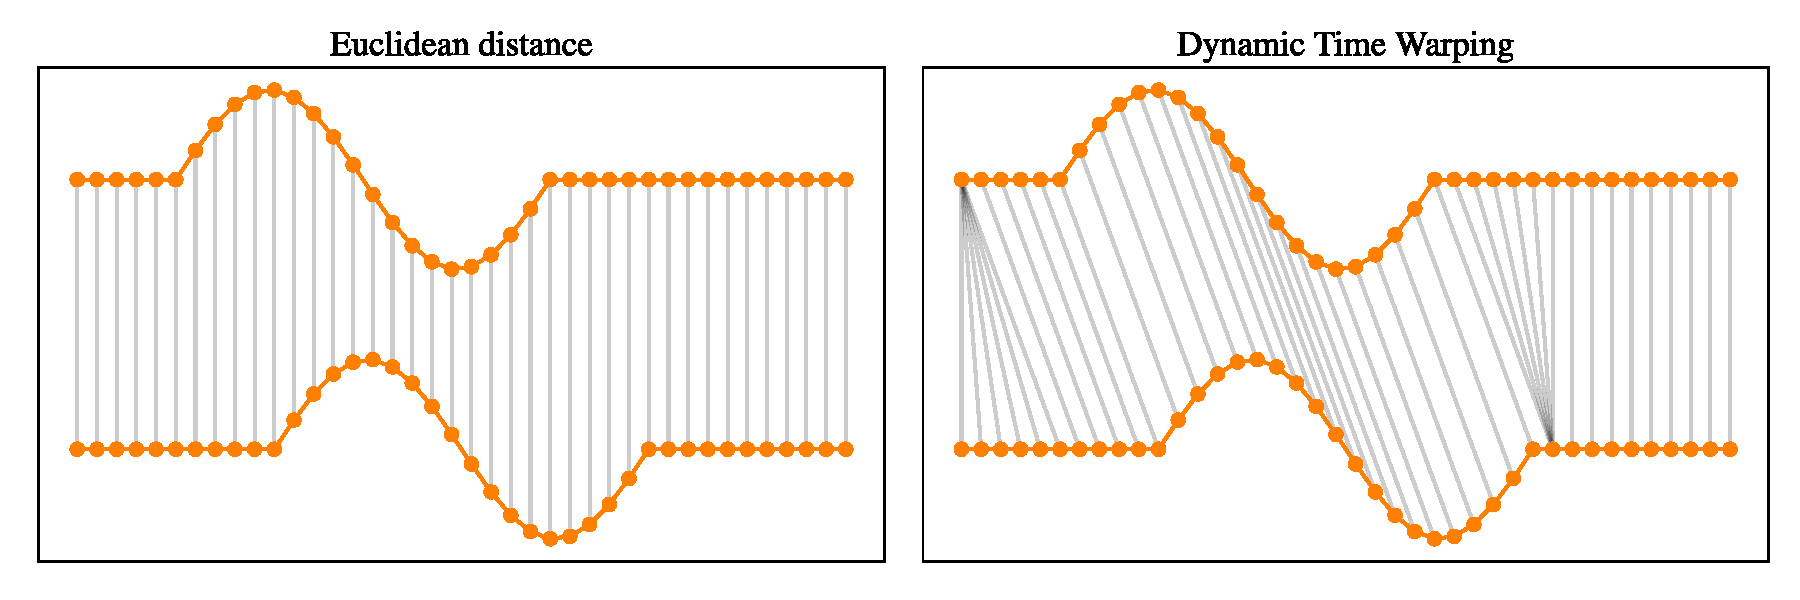
\includegraphics[width=\textwidth]{results/dtw_vs_euc}
    \caption{Comparison between DTW and Euclidean distance, adapted from \cite{tavenard.blog.dtw}}
    \label{fig:dtw_vs_euc}
\end{figure}

\subsection{Round-Trip Time}
The Round-Trip Time is the time that elapses between the moment a status is sent from the vehicle to the operator and the instruction calculated on that status is received.

\subsection{Channel Quality Indicator}
The Channel Quality Indicator (CQI) is a numerical value between 0 and 15 that describes how good the communication channel is, with 0 being the worst and 15 being the best value. A bad quality channel forces the use of modulation coding schemes that are more resistant to data corruption but less efficient in terms of data rates. It also increases the chance of needing to make retransmissions because of corrupt frames, which in turn increases the network delay and bandwidth usage.

\subsection{Resource Block Utilization percentage}
This is the percentage of available physical resource blocks that the vehicle uses in transmitting its status and sensor data.

%\pagebreak
\section{City trip}
As introduced in Section \ref{subsec:scenarios:city_trip:background}, this route was considered with both static background and moving background simulation models.

In this context, the completion percentage across the 10 runs for each scenario will be plotted as bars colored in green for the successful share of runs and red for the share of failed runs.

Trajectory error, RTT, CQI, and RB utilization percentage will be traced as subplots sharing the same x-axis corresponding to the distance from the origin point. Vertical dotted lines are placed in correspondence with the handover from one base station to another.

\subsection{Static background}

\begin{figure}[H]
    \centering
    \begin{subfigure}[b]{0.95\textwidth}
        \centering
        \includegraphics[width=\textwidth]{results/valerios_sim_fixed_numerology/simulation_status_25}
        \caption{25 fps}
    \end{subfigure}
    \hfill
    \begin{subfigure}[b]{0.95\textwidth}
        \centering
        \includegraphics[width=\textwidth]{results/valerios_sim_fixed_numerology/simulation_status_60}
        \caption{60 fps}
    \end{subfigure}
    \caption{City trip with static background - Simulations completion percentage}
    \label{fig:valerios_sim_fixed_numerology_completion_percentage}
\end{figure}

\figurename~\ref{fig:valerios_sim_fixed_numerology_completion_percentage} shows an overall look at the completion percentage across the 10 runs executed over each of the 32 considered parameter configurations.


This route and parameter configuration is very similar to what is described in \cite{valeriopaper}, with the difference being that the change in the resource block allocation to keep constant bandwidth across all runs made it impossible for the scenarios with 66kB status packet size and 60fps refresh rate to be successfully completed, regardless of numerology and number of background sources, as in the configurations with a numerology parameter $\mu$ of 1 the Host Vehicle no longer had double the amount of bandwidth available to it.

\begin{figure}[H]
    \centering
    \includegraphics[width=\textwidth]{results/valerios_sim_fixed_numerology/err_rtt_cqi_rb_25_0}
    \caption{City trip with no background - Trajectory error, RTT, CQI, and allocated resource blocks over distance from origin, 25~fps}
    \label{fig:valerios_sim_fixed_numerology_err_rtt_cqi_rb_25_0}
\end{figure}

\figurename~\ref{fig:valerios_sim_fixed_numerology_err_rtt_cqi_rb_25_0} traces the trajectory error, RTT, CQI and used RBs in the absence of background for scenarios with packet size of 33 and 66kB, numerology of 0 and 1 and 25fps, each averaged over the respective 10 runs. The error on the trajectory spikes in correspondence with the more difficult parts of the route, i.e.\ the sections with curves.
It can be observed that the dips in channel quality make both the RTT and the percentage of used RBs increase. This is because as channel quality lowers the frequency of corrupted or dropped packets increases and thus more bandwidth is required and a delay occurs.

\begin{figure}[H]
    \centering
    \includegraphics[width=\textwidth]{results/valerios_sim_fixed_numerology/err_rtt_cqi_rb_25_3}
    \caption{City trip with 3 static background users - Trajectory error, RTT, CQI, and allocated resource blocks over distance from origin, 25~fps}
    \label{fig:valerios_sim_fixed_numerology_err_rtt_cqi_rb_25_3}
\end{figure}

\figurename~\ref{fig:valerios_sim_fixed_numerology_err_rtt_cqi_rb_25_3} traces the trajectory error, RTT, CQI and used RBs in the presence of 3 background users near each base station for scenarios with packet size of 33 and 66kB, numerology of 0 and 1 and 25fps. Here the trajectory error is basically the same as the previous set of plots but the RTT and used RBs are showing an increase. This is a consequence of the background users' activity on the network, but still within the margins for safe operation.

\begin{figure}[H]
    \centering
    \includegraphics[width=\textwidth]{results/valerios_sim_fixed_numerology/err_rtt_cqi_rb_60_3}
    \caption{City trip with 3 static background users - Trajectory error, RTT, CQI, and allocated resource blocks over distance from origin, 60~fps}
    \label{fig:valerios_sim_fixed_numerology_err_rtt_cqi_rb_60_3}
\end{figure}

\figurename~\ref{fig:valerios_sim_fixed_numerology_err_rtt_cqi_rb_60_3} traces the trajectory error, RTT, CQI and used RBs in the presence of 3 background users near each base station for scenarios with packet size of 33kB, numerology of 0 and 1 and 60fps. The scenarios with a 66kB packet size are absent as each of their repetitions failed. The RTT is within safe values and in fact the trajectory error is also on the safe side. The percentage of used RBs is nearing full utilization in the sections of the route with lower channel quality. This gives a hint towards the reason why the scenarios with a bigger packet size failed.

\begin{figure}[H]
    \centering
    \includegraphics[width=\textwidth]{results/valerios_sim_fixed_numerology/failed_err_rtt_cqi_rb}
    \caption{City trip with static background failed runs - Trajectory error, RTT, CQI, and allocated resource blocks over distance from origin}
    \label{fig:valerios_sim_fixed_numerology_failed_err_rtt_cqi_rb_60_3}
\end{figure}


\figurename~\ref{fig:valerios_sim_fixed_numerology_failed_err_rtt_cqi_rb_60_3} traces the trajectory error, RTT, CQI and used RBs for the scenarios where the simulations failed, i.e.\ a crash occurred. This happened at the start of the simulation and the main culprit is the complete exhaustion of the available amount of Resource Blocks in conjunction with the dwindling channel quality. The RTT skyrockets, the ToD operator is unable to keep control of the vehicle and a crash is inevitable.



\subsection{Moving background}
\begin{figure}[H]
    \centering
    \begin{subfigure}[b]{0.95\textwidth}
        \centering
        \includegraphics[width=\textwidth]{results/original_city_trip_movingbg/simulation_status_25}
        \caption{25 fps}
    \end{subfigure}
    \hfill
    \begin{subfigure}[b]{0.95\textwidth}
        \centering
        \includegraphics[width=\textwidth]{results/original_city_trip_movingbg/simulation_status_60}
        \caption{60 fps}
    \end{subfigure}
    \caption{City trip with moving background - Simulations completion percentage}
    \label{fig:original_city_trip_movingbg_completion_percentage}
\end{figure}

\figurename~\ref{fig:original_city_trip_movingbg_completion_percentage} shows an overall look at the completion percentage across the 10 runs executed over each of the 32 considered parameter configurations.

The difference from the previous section is the nature of the background users, so the scenario with no background corresponds to the one in \figurename~\ref{fig:valerios_sim_fixed_numerology_err_rtt_cqi_rb_25_0}.

\begin{figure}[H]
    \centering
    \includegraphics[width=\textwidth]{results/original_city_trip_movingbg/err_rtt_cqi_rb_25_3}
    \caption{City trip with 3 moving background users - Trajectory error, RTT, CQI, and allocated resource blocks over distance from origin, 25~fps}
    \label{fig:original_city_trip_movingbg_err_rtt_cqi_rb_25_3}
\end{figure}

\figurename~\ref{fig:original_city_trip_movingbg_err_rtt_cqi_rb_25_3} traces the trajectory error, RTT, CQI and used RBs in the presence of 3 moving background users for scenarios with packet size of 33 and 66kB, numerology of 0 and 1 and 25fps.

\begin{figure}[H]
    \centering
    \includegraphics[width=\textwidth]{results/original_city_trip_movingbg/err_rtt_cqi_rb_60_3}
    \caption{City trip with 3 moving background users - Trajectory error, RTT, CQI, and allocated resource blocks over distance from origin, 60~fps}
    \label{fig:original_city_trip_movingbg_err_rtt_cqi_rb_60_3}
\end{figure}

\figurename~\ref{fig:original_city_trip_movingbg_err_rtt_cqi_rb_60_3} traces the trajectory error, RTT, CQI and used RBs in the presence of 3 moving background users for scenarios with packet size of 33kB, numerology of 0 and 1 and 60fps. The scenarios with a 66kB packet size are absent as each of their repetitions failed.

It is noticeable that the moving background users make the network conditions much more challenging and unpredictable. This is because as they are traveling, though around the same area as the Host Vehicle, they will need to switch base stations and will each experience varying channel quality with its consequences. In both figures towards the end of the route the amount of used RBs almost tops out, leading to the danger of a crash.

The effect of randomness is observable in the failures experienced in some scenarios where in theory the available resources are enough, as 90\% of the runs succeeded, but still there was a crash due to a sudden spike in latency, likely influenced by unforeseen conditions that the network couldn't efficiently handle.

\begin{figure}[H]
    \centering
    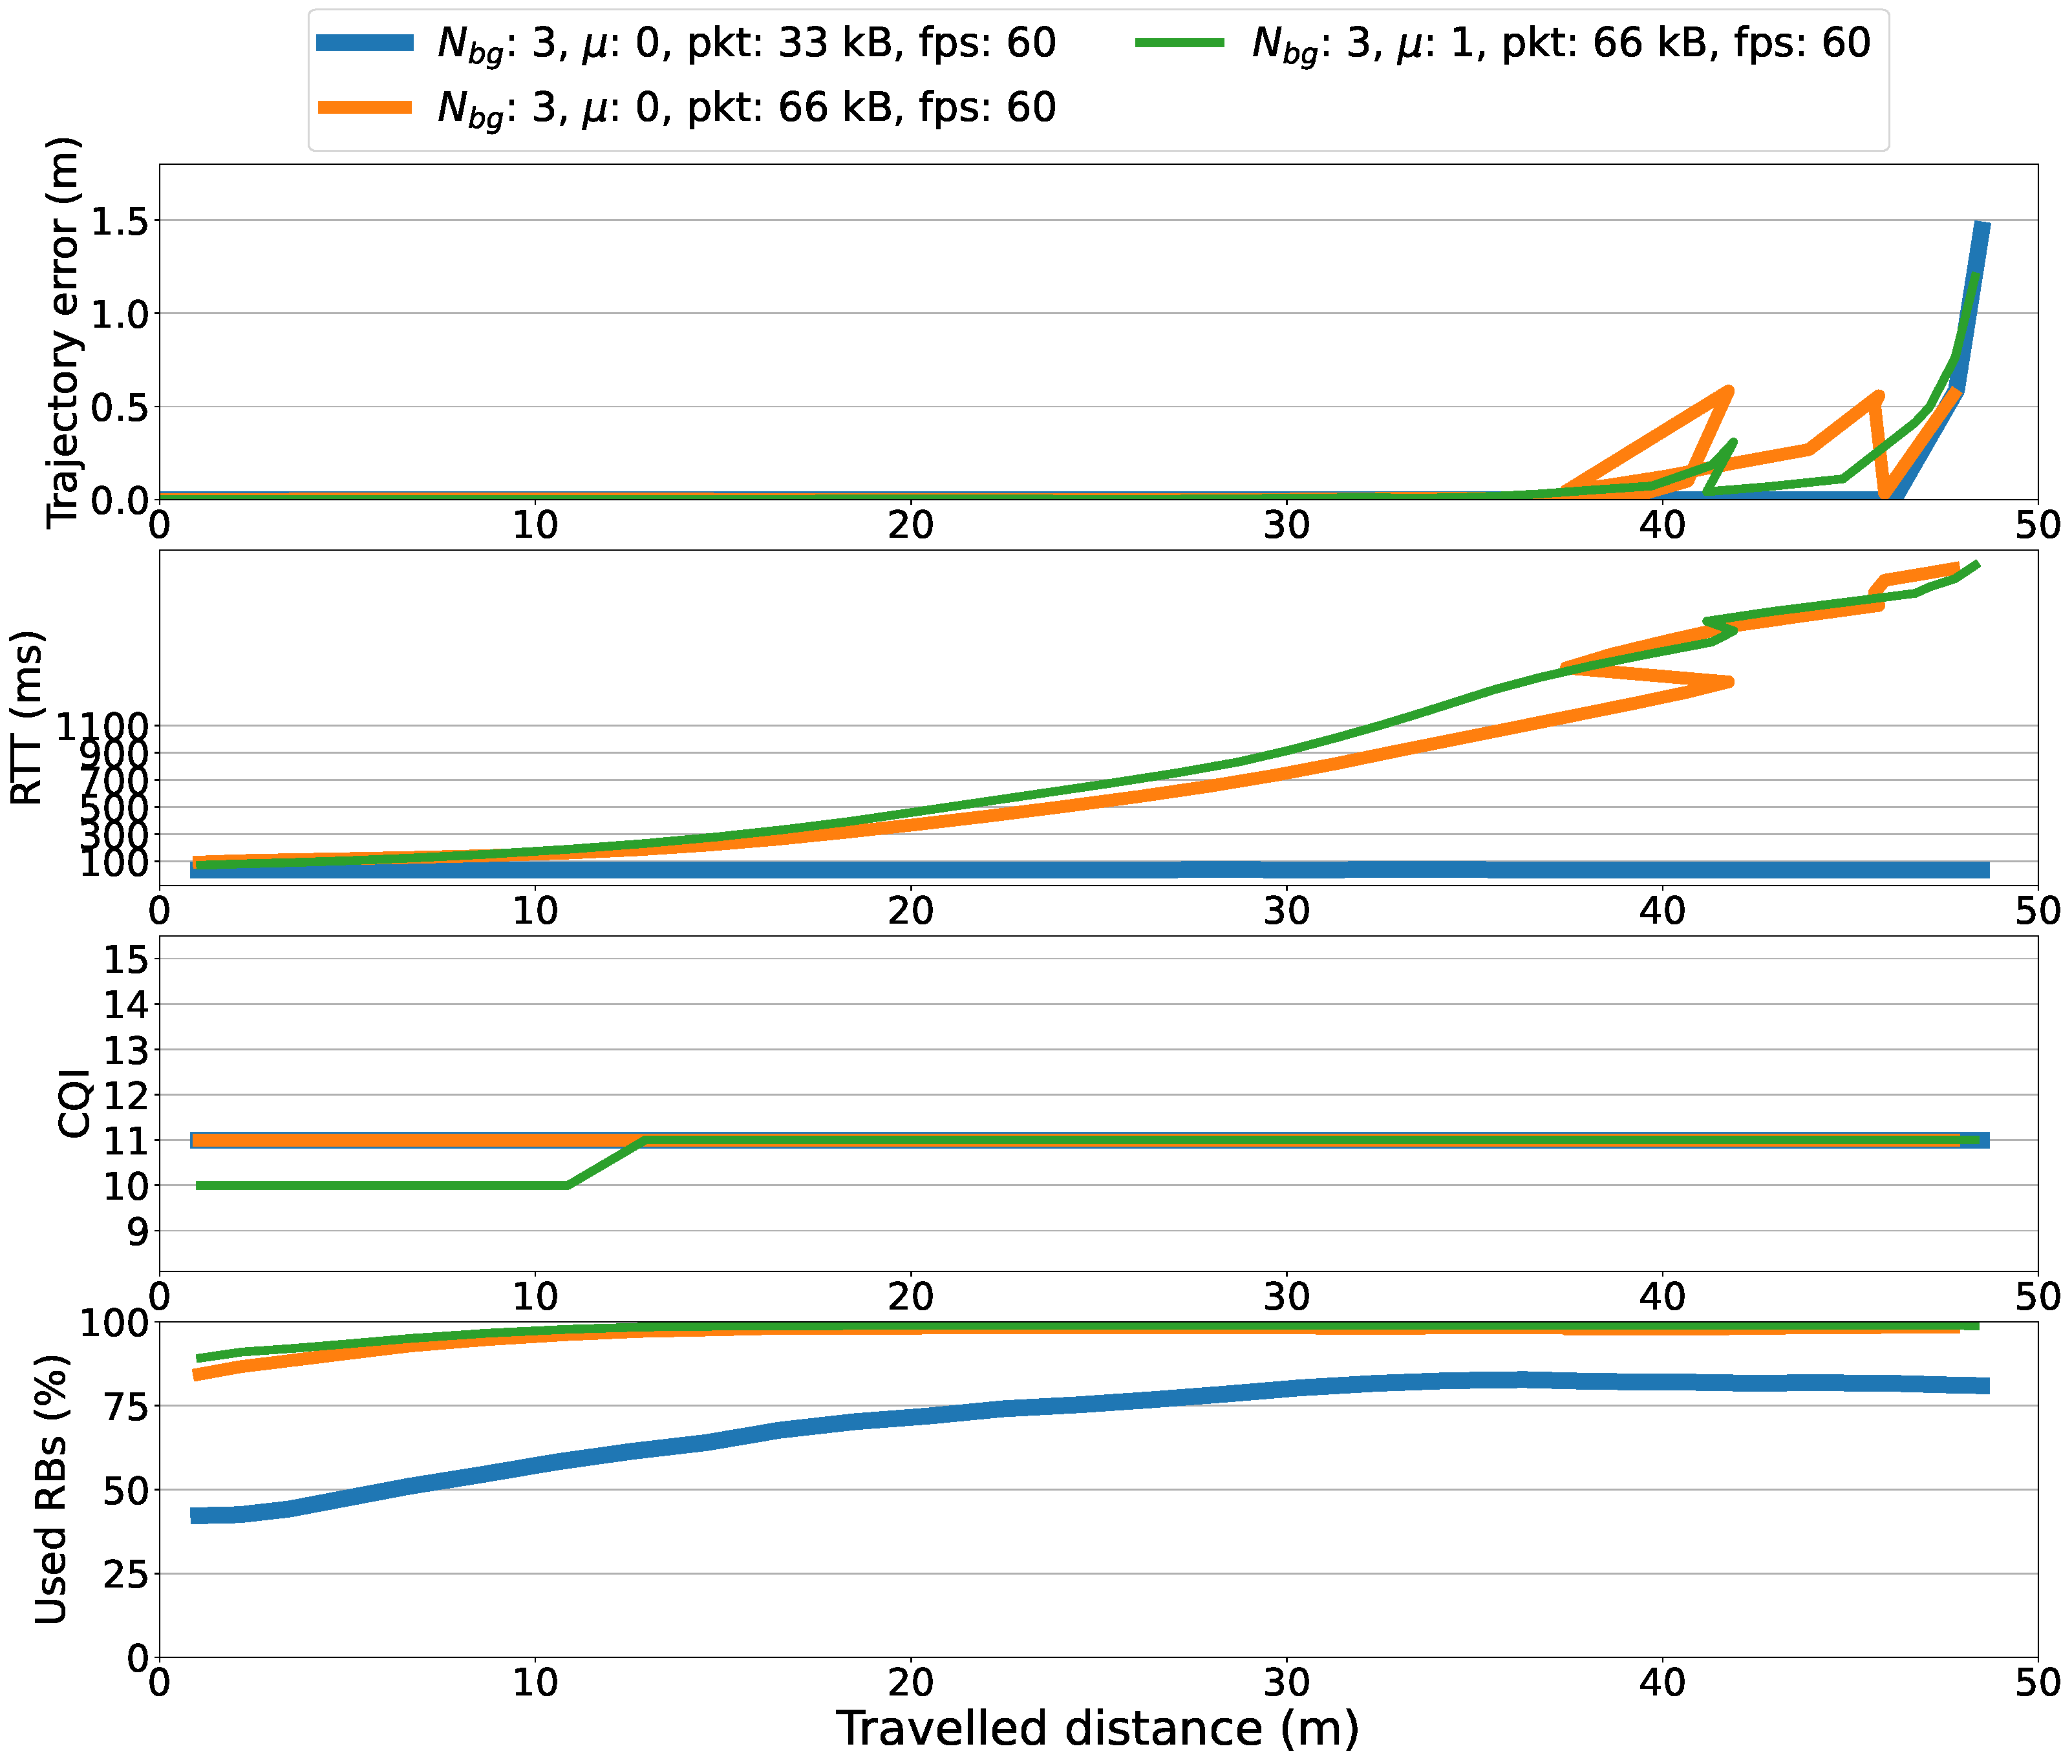
\includegraphics[width=\textwidth]{results/original_city_trip_movingbg/failed_err_rtt_cqi_rb_60_3}
    \caption{City trip with moving background failed runs - Trajectory error, RTT, CQI, and allocated resource blocks over distance from origin}
    \label{fig:original_city_trip_movingbg_failed_err_rtt_cqi_rb_60_3}
\end{figure}

\figurename~\ref{fig:original_city_trip_movingbg_failed_err_rtt_cqi_rb_60_3} traces the trajectory error, RTT, CQI and used RBs for the scenarios where the simulations failed. As was the case before, these configurations are the most demanding ones in terms of data rate and QoS, hence the result is the same: the amount of used RBs goes to 100\% from the start and the operator loses control right away.






% \begin{figure}[H]
%     \centering
%     \includegraphics[width=\textwidth]{results/original_city_trip_movingbg/err_rtt_cqi_rb_25_0}
%     \caption{City trip with moving background - Trajectory error, RTT, CQI, and allocated resource blocks over distance from origin with 0 ToD services background, and 25~fps}
%     \label{fig:original_city_trip_movingbg_err_rtt_cqi_rb_25_0}
% \end{figure}








\pagebreak

\section{Reaction to obstacles}
This section contains the results of the experiments conducted in the presence of obstacles. In the case of a city context, both obstacles present from the start and suddenly appearing were tested. For the highway scenarios, only the latter option was chosen.

As was the case for the city trip results, the completion percentage for each scenario will be plotted as bars colored in green for the successful share of runs and red for the share of failed runs.

The following 4-subplot configuration (e.g.\ in \figurename~\ref{fig:city_static_obstacle_err_rtt_cqi_rb_60_3}) resembles the one described for the city trips, the only difference being that since the trajectory error is not meaningful in such scenarios as the ones involving obstacles, the first subplot instead traces the distance to the obstacle location (when present in the world).

The distance to the obstacle, RTT, CQI and RB utilization percentage will be traced as subplots sharing the same x-axis corresponding to the distance from the origin point. In some cases, the plots will be trimmed not to start from the exact origin in order to better emphasize the important section which is towards the end, where the obstacle is.


\subsection{Static obstacle}

\begin{figure}[H]
    \centering
    \begin{subfigure}[b]{0.95\textwidth}
        \centering
        \includegraphics[width=\textwidth]{results/city_static_obstacle/simulation_status_25}
        \caption{25 fps}
    \end{subfigure}
    \hfill
    \begin{subfigure}[b]{0.95\textwidth}
        \centering
        \includegraphics[width=\textwidth]{results/city_static_obstacle/simulation_status_60}
        \caption{60 fps}
    \end{subfigure}
    \caption{City static obstacle - Simulations completion percentage}
    \label{fig:city_static_obstacle_completion_percentage}
\end{figure}

\figurename~\ref{fig:city_static_obstacle_completion_percentage} shows an overall look at the completion percentage across the 10 runs executed over each of the 32 considered scenarios.
The reason why this test was not repeated for the highway case is that, as the results show, there is almost no situation where a collision cannot be avoided. There were a couple of cases where a collision indeed occurred and they were all a small number of runs for the scenarios with the most load on the network which would make even a simple turn in the road impossible while using ToD.

\begin{figure}[H]
    \centering
    \includegraphics[width=\textwidth]{results/city_static_obstacle/err_rtt_cqi_rb_60_3}
    \caption{City static obstacle with 3 background users - Distance to obstacle, RTT, CQI, and allocated resource blocks over distance from origin, 60~fps}
    \label{fig:city_static_obstacle_err_rtt_cqi_rb_60_3}
\end{figure}

\figurename~\ref{fig:city_static_obstacle_err_rtt_cqi_rb_60_3} traces the distance to obstacle, RTT, CQI and used RBs in the presence of 3 background users per base station for scenarios with packet size of 33kB and 66kB, numerology of 0 and 1 and 60fps, i.e.\ the most demanding scenarios, for runs that did not fail. The scenarios with the bigger packet size saturate the available resource blocks and the latency goes off the charts. Nevertheless, at least some instructions go through and a collision is avoided.

\begin{figure}[H]
    \centering
    \includegraphics[width=\textwidth]{results/city_static_obstacle/failed_err_rtt_cqi_rb}
    \caption{City static obstacle failed runs - Distance to obstacle, RTT, CQI, and allocated resource blocks over distance from origin}

    \label{fig:city_static_obstacle_failed_err_rtt_cqi_rb}
\end{figure}

\figurename~\ref{fig:city_static_obstacle_failed_err_rtt_cqi_rb} shows the same metrics for the very few failed runs. These are the only cases where, even when the obstacle is observed from afar, the strain on the network is so much that the ToD operator is unable to stop the vehicle.



% \begin{figure}[H]
%     \centering
%     \includegraphics[width=\textwidth]{results/city_static_obstacle/err_rtt_cqi_rb_25_0}
%     \caption{City static obstacle - Distance to obstacle, RTT, CQI, and allocated resource blocks over distance from origin with 0 ToD services background, and 25~fps}
%     \label{fig:city_static_obstacle_err_rtt_cqi_rb_25_0}
% \end{figure}

% \begin{figure}[H]
%     \centering
%     \includegraphics[width=\textwidth]{results/city_static_obstacle/err_rtt_cqi_rb_25_3}
%     \caption{City static obstacle - Distance to obstacle, RTT, CQI, and allocated resource blocks over distance from origin with 3 ToD services background, and 25~fps}
%     \label{fig:city_static_obstacle_err_rtt_cqi_rb_25_3}
% \end{figure}


\pagebreak
\subsection{City sudden obstacle}
The sudden obstacle scenarios tell a much more interesting story. 

\begin{figure}[H]
    \centering
    \begin{subfigure}[b]{0.95\textwidth}
        \centering
        \includegraphics[width=\textwidth]{results/city_sudden_obstacle/simulation_status_25}
        \caption{25 fps}
    \end{subfigure}
    \hfill
    \begin{subfigure}[b]{0.95\textwidth}
        \centering
        \includegraphics[width=\textwidth]{results/city_sudden_obstacle/simulation_status_60}
        \caption{60 fps}
    \end{subfigure}
    \caption{City sudden obstacle - Simulations completion percentage}
    \label{fig:city_sudden_obstacle_completion_percentage}
\end{figure}

\figurename~\ref{fig:city_sudden_obstacle_completion_percentage} illustrates the completion rate for each scenario and the most noticeable pattern is that the right side of both subfigures is much greener overall than the left, the difference being the numerology index $\mu$, which is 0 on the left and 1 on the right. The only exception is for those scenarios where the bandwidth is saturated.

\begin{figure}[H]
    \centering
    \includegraphics[width=\textwidth]{results/city_sudden_obstacle/err_rtt_cqi_rb_25_0}
    \caption{City sudden obstacle with no background - Distance to obstacle, RTT, CQI, and allocated resource blocks over distance from origin, 25~fps}
    \label{fig:city_sudden_obstacle_err_rtt_cqi_rb_25_0}
\end{figure}

\figurename~\ref{fig:city_sudden_obstacle_err_rtt_cqi_rb_25_0} traces the distance to obstacle, RTT, CQI and used RBs in the absence of background for scenarios with packet size of 33 and 66kB, numerology of 0 and 1 and 25fps, each averaged over the respective successful runs.

\begin{figure}[H]
    \centering
    \includegraphics[width=\textwidth]{results/city_sudden_obstacle/err_rtt_cqi_rb_25_3}
    \caption{City sudden obstacle with 3 background users - Distance to obstacle, RTT, CQI, and allocated resource blocks over distance from origin, 25~fps}
    \label{fig:city_sudden_obstacle_err_rtt_cqi_rb_25_3}
\end{figure}

\figurename~\ref{fig:city_sudden_obstacle_err_rtt_cqi_rb_25_3} traces the distance to obstacle, RTT, CQI and used RBs in the presence of 3 background users for scenarios with packet size of 33 and 66kB, numerology of 0 and 1 and 25fps.

\begin{figure}[H]
    \centering
    \includegraphics[width=\textwidth]{results/city_sudden_obstacle/err_rtt_cqi_rb_60_3}
    \caption{City sudden obstacle with 3 background users - Distance to obstacle, RTT, CQI, and allocated resource blocks over distance from origin, 60~fps}
    \label{fig:city_sudden_obstacle_err_rtt_cqi_rb_60_3}
\end{figure}

\figurename~\ref{fig:city_sudden_obstacle_err_rtt_cqi_rb_60_3} traces the distance to obstacle, RTT, CQI and used RBs in the presence of 3 background users for scenarios with packet size of 33 and 66kB, numerology of 0 and 1 and 60fps. It can be noticed that for the 66kB scenarios the absence of a crash was a stroke of luck, as the resource block utilization is pegged at 100\% and the delay is completely out of range for safe operation. In fact, the successful runs make up a minority of the 10 runs for each scenario.

\begin{figure}[H]
    \centering
    \includegraphics[width=\textwidth]{results/city_sudden_obstacle/failed_err_rtt_cqi_rb}
    \caption{City sudden obstacle failed runs - Distance to obstacle, RTT, CQI, and allocated resource blocks over distance from origin}
    \label{fig:city_sudden_obstacle_failed_err_rtt_cqi_rb_60_3}
\end{figure}

\figurename~\ref{fig:city_sudden_obstacle_failed_err_rtt_cqi_rb_60_3} traces the distance to obstacle, RTT, CQI and used RBs for a selection of the failed runs. For cases where the resource block utilization and RTT are within regular margin, the failures have to do with the slight variance of network conditions across different random seeds in a situation where timing is very tight. The trend is apparent in the overall success/failure rates. For the rest of the scenarios, it is evident that since the channel is saturated and packets pile up, it is impossible for data to be exchanged with the vehicle and stop it in time.


\pagebreak

\subsection{Highway sudden obstacle}

\begin{figure}[H]
    \centering
    \begin{subfigure}[b]{0.95\textwidth}
        \centering
        \includegraphics[width=\textwidth]{results/hwy_sudden_obstacle/simulation_status_25}
        \caption{25 fps}
    \end{subfigure}
    \hfill
    \begin{subfigure}[b]{0.95\textwidth}
        \centering
        \includegraphics[width=\textwidth]{results/hwy_sudden_obstacle/simulation_status_60}
        \caption{60 fps}
    \end{subfigure}
    \caption{Highway sudden obstacle - Simulations completion percentage}
    \label{fig:hwy_sudden_obstacle_completion_percentage}
\end{figure}

\figurename~\ref{fig:hwy_sudden_obstacle_completion_percentage} illustrates the completion rate for each scenario and the same considerations as the city context hold true: scenarios with numerology index $\mu$ of 1 have a higher success rate even as the available bandwidth stays the same because of the overall lower RTT.

It is worth noting that the selected spawn distance of 44 meters was purposely chosen as an \textit{edge case}, which shows that in tight circumstances even a few milliseconds of added or reduced delay will make a difference. However, the same tests repeated using a distance of 45 meters yielded an almost completely successful set of simulations.

\begin{figure}[H]
    \centering
    \includegraphics[width=\textwidth]{results/hwy_sudden_obstacle/err_rtt_cqi_rb_25_0}
    \caption{Highway sudden obstacle with no background - Distance to obstacle, RTT, CQI, and allocated resource blocks over distance from origin, 25~fps}
    \label{fig:hwy_sudden_obstacle_err_rtt_cqi_rb_25_0}
\end{figure}

\figurename~\ref{fig:hwy_sudden_obstacle_err_rtt_cqi_rb_25_0} traces the distance to obstacle, RTT, CQI and used RBs in the absence of background for scenarios with packet size of 33 and 66kB, numerology of 0 and 1 and 25fps, each averaged over the respective successful runs.

\begin{figure}[H]
    \centering
    \includegraphics[width=\textwidth]{results/hwy_sudden_obstacle/err_rtt_cqi_rb_25_3}
    \caption{Highway sudden obstacle with 3 background users - Distance to obstacle, RTT, CQI, and allocated resource blocks over distance from origin, 25~fps}
    \label{fig:hwy_sudden_obstacle_err_rtt_cqi_rb_25_3}
\end{figure}

\figurename~\ref{fig:hwy_sudden_obstacle_err_rtt_cqi_rb_25_3} traces the distance to obstacle, RTT, CQI and used RBs in the presence of 3 background users for scenarios with packet size of 33 and 66kB, numerology of 0 and 1 and 25fps.

\begin{figure}[H]
    \centering
    \includegraphics[width=\textwidth]{results/hwy_sudden_obstacle/err_rtt_cqi_rb_60_3}
    \caption{Highway sudden obstacle with 3 background users - Distance to obstacle, RTT, CQI, and allocated resource blocks over distance from origin, 60~fps}
    \label{fig:hwy_sudden_obstacle_err_rtt_cqi_rb_60_3}
\end{figure}

\figurename~\ref{fig:hwy_sudden_obstacle_err_rtt_cqi_rb_60_3} traces the distance to obstacle, RTT, CQI and used RBs in the presence of 3 background users for scenarios with packet size of 33 and 66kB, numerology of 0 and 1 and 60fps. Differently from the previous context, the resource block utilization on average doesn't tend to saturate just as much, likely because of the slightly higher channel quality, but still it's not at a level that would tolerate much variation in the network conditions.

\begin{figure}[H]
    \centering
    \includegraphics[width=\textwidth]{results/hwy_sudden_obstacle/failed_err_rtt_cqi_rb}
    \caption{Highway sudden obstacle failed runs - Distance to obstacle, RTT, CQI, and allocated resource blocks over distance from origin}
    \label{fig:hwy_sudden_obstacle_failed_err_rtt_cqi_rb_60_3}
\end{figure}

\figurename~\ref{fig:hwy_sudden_obstacle_failed_err_rtt_cqi_rb_60_3} traces the distance to obstacle, RTT, CQI and used RBs for a selection of the failed runs. It shows that there were failures for all levels of network load and delay, once again influenced by randomness.


%IN QUESTO PUNTO AGGIUNGEREI UNA DISCUSSIONE FINALE 
\section{Discussion}
The simulation results have shown that Tele-Operated Driving is a possibility under the right circumstances and with the right setup. With a 20MHz bandwidth available and especially with other users impacting the shared medium, it is important to mind the data rates of the video feeds and the refresh rate of the information sent to the remote ToD operator.

The most impactful parameter has been the Round-Trip Time calculated as the time between the detection of the environment by the sensors on the HV and the corresponding instruction issued back by the ToD operator based on that data. The more it increases the more disconnected the Operator is from reality time-wise and the harder it is for them to keep a steady control of the vehicle, avoiding drifting too much from the predetermined trajectory and eventually crashing into a wall or not stopping in time for a sudden emergency.

The RTT is greatly influenced by the load posed on the network by the HV itself and by other users. The channel quality also has an impact in the choice of more or less efficient modulation schemes thus impacting the effective maximum throughput at any given time. The varying distance from the base station and subsequent handover to a closer one when moving around the world are also critical. An exhaustion of the available network resources must be avoided as continuous communication is vital for a successful execution of the remote driving tasks.

Overall, configurations with a numerology index $\mu$ of 1 have proven to be more reliable, because of its generally lower delay in exchanging data and instructions, especially in the sudden obstacle scenarios where even a reduction in latency of a few milliseconds makes a big difference.